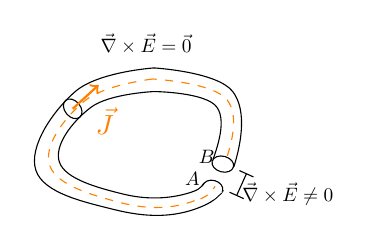
\begin{tikzpicture}
\draw  plot[smooth, tension=.7] coordinates {(0,0.8) (-1,0.5) (-1.5,-0.5) (-0.5,-1) (0.5,-1) (1,-0.5) (1,0.5) (0,0.8)};
\draw  plot[smooth, tension=.7] coordinates {(0,0.5) (-0.8,0.3) (-1.2,-0.4) (-0.4,-0.8) (0.4,-0.8) (0.7,-0.5) (0.8,0.3) (0,0.5)};
\draw [rotate=40] (-0.6105,0.8787) node (v1) {} ellipse (0.1 and 0.14);
\draw [->, thick, orange](v1.center) -- (-0.703,0.583) node[midway, below right]{$\vec{J}$};
\node at (-0.1,1.1) [scale=0.7]{$\vec{\nabla}\times \vec{E}=\vec{0}$};
\node [scale=0.7] at (1.7,-0.8) {$\vec{\nabla}\times \vec{E}\neq0$};
\draw  [dashed, orange]plot[smooth, tension=.7] coordinates {(-0.0165,0.6592) (-0.8872,0.376) (-1.3237,-0.4412) (-0.4367,-0.9078) (0.4525,-0.9078) (0.8726,-0.4876) (0.9284,0.3946) (-0.0165,0.6592)};
\draw [fill, white, rotate=-20] (0.6033,-0.0883) rectangle (1.2,-0.4);
\draw  [rotate=-15](0.9535,-0.1806) ellipse (0.14 and 0.1);
\draw  [rotate=-15](0.9088,-0.51) ellipse (0.13 and 0.1);
\draw [fill, white](0.5704,-0.7592) node (v2) {} -- (0.6528,-0.6823) -- (0.8552,-0.7752) -- (0.7572,-0.8614) -- (v2.center);
\node at (0.4885,-0.6108) [scale=0.7]{$A$};
\node [scale=0.7] at (0.671,-0.3307) {$B$};
\draw [|-|](1.0471,-0.8257) -- (1.177,-0.5376);
\draw [fill, white] (0.5557,-0.8143) rectangle (0.6707,-0.8843);
\draw [dashed, orange] plot[smooth, tension=.7] coordinates {(0.5907,-0.8643) (0.7007,-0.7993) (0.7757,-0.7043)};
\end{tikzpicture}
